%\documentclass[hyperref={pdfpagelabels=false},slidetop,9pt]{beamer}
\documentclass[slidetop,8pt]{beamer}
\usepackage[T1]{fontenc}
\usepackage[utf8]{inputenc}
\newcommand{\id}{54}
\newcommand{\nom}{Liaisons mécaniques}
\newcommand{\sequence}{04}
\newcommand{\num}{01}
\newcommand{\type}{TP}
\newcommand{\descrip}{Modélisation d'un solide. Comportement des liaisons mécaniques. Modéliser les mécanismes du laboratoire par un schéma cinématique, paramétré.}
\newcommand{\competences}{A3-C4: Analyse d'architecture et de comportement \\ &  Mod1-C1: Isolement d'un solide ou d'un système de solides \\ &  Mod2-C10-1: Modèle de solide indéformable \\ &  Mod2-C11: Modélisation géométrique et cinématique des mouvements entre solides indéformables \\ &  Mod2-C12: Modélisation cinématique des liaisons entre solides \\ &  Mod2-C15: Modélisation des actions mécaniques \\ &  Rés-C6: Utilisation d'un solveur ou d'un logiciel multi physique \\ &  Com1-C1: Différents descripteurs introduits dans le programme \\ &  Com2-C4: Outils de communication}
\newcommand{\nbcomp}{9}
\newcommand{\systemes}{Plateforme Stewart}
\newcommand{\systemessansaccent}{Plateforme Stewart}
\newcommand{\ilot}{2}
\newcommand{\ilotstr}{02}
\newcommand{\dossierilot}{\detokenize{Ilot_02 Plateforme Stewart}}
\newcommand{\imageun}{Plateforme}

\newcommand{\urlsysteme}{\href{https://www.costadoat.fr/systeme/57}{Ressources système}}
\newcommand{\matlabsimscape}{\href{https://github.com/Costadoat/Sciences-Ingenieur/raw/master/Systemes/Plateforme Stewart/Plateforme_Stewart_Simscape.zip}{Modèle Simscape}}
\newcommand{\solidworks}{\href{https://github.com/Costadoat/Sciences-Ingenieur/raw/master/Systemes/Plateforme Stewart/Plateforme_Stewart_Solidworks.zip}{Modèle Solidworks}}
\newcommand{\edrawings}{\href{https://github.com/Costadoat/Sciences-Ingenieur/raw/master/Systemes/Plateforme Stewart/Plateforme_Stewart.EASM}{Modèle eDrawings}}
\newcommand{\test}{Stewart_param1}
\newcommand{\testi}{Stewart_param2}
\newcommand{\testii}{Stewart_param3}
\newcommand{\testiii}{Stewart_param4}
\newcommand{\testiiii}{Stewart_euler}
\usepackage{etex}
\usepackage{tikz}
\usepackage[european]{circuitikz}
\usepackage{pgf}
\usepackage[all]{xy}
\usepackage{pgfpages}
\usepackage{graphbox}
\usepackage{pdfpages}
\usepackage[adobe-utopia]{mathdesign}
\usepackage{ifthen}
\usepackage{cancel}
\usepackage{framed}
\usepackage{subfig}
\usepackage{tabularx}
\usepackage{setspace}
\usepackage{soul}
\usepackage{schemabloc}
\usepackage{eqnarray}
\usepackage[dot, phantomtext]{dashundergaps}
\usepackage{media9}
\usepackage{multimedia}
\usepackage{textcomp}

\author{Renaud Costadoat}
\institute{Lycée Dorian}

\usepackage{multido}
\usepackage{multirow}
\usepackage{multicol} % Portions de texte en colonnes
\usepackage{flafter}%floatants après la référence

\usepackage{color}
\usepackage{xcolor}
\usepackage{colortbl}

\usepackage[gen]{eurosym}
\usepackage{tikz}
%\usepackage{pstricks,pst-node,pst-tree,pst-solides3d}
\usepackage{lmodern}
\usepackage[francais]{babel}
\usepackage{pslatex}
\usetheme{renaud}
\usepackage{times}
\usepackage{amsmath}
\usepackage{verbatim}
\usepackage{moreverb}
%\usetikzlibrary{arrows,shapes}
\usepackage{graphicx}
\usepackage{psfrag}
\usepackage{wrapfig}
\usepackage{etoolbox}

\definecolor{gris25}{gray}{0.75}
\definecolor{bleu}{RGB}{18,33,98}
\definecolor{bleuf}{RGB}{42,94,171}
\definecolor{bleuc}{RGB}{231,239,247}
\definecolor{rougef}{RGB}{185,18,27}
\definecolor{rougec}{RGB}{255,188,204}%255,230,231
\definecolor{vertf}{RGB}{103,126,82}
\definecolor{vertc}{RGB}{220,255,191}

\setlength\parindent{24pt}
\parskip 7.2pt
\parindent 8pt

\newenvironment{rem}[1][\hsize]%
{%
    \def\FrameCommand
   {%
\rotatebox{90}{\textit{\textsf{Remarque}}} 
       {\color{bleuf}\vrule width 3pt}%
       \hspace{0pt}%must no space.
       \fboxsep=\FrameSep\colorbox{bleuc}%
  }%
    \MakeFramed{\hsize#1\advance\hsize-\width\FrameRestore}%
}%
{\endMakeFramed}%


\newenvironment{savoir}[1][\hsize]%
{%
    \def\FrameCommand
    {%
\rotatebox{90}{\textit{\textsf{Savoir}}} 
        {\color{bleuf}\vrule width 3pt}%
        \hspace{0pt}%must no space.
        \fboxsep=\FrameSep\colorbox{bleuc}%
    }%
    \MakeFramed{\hsize#1\advance\hsize-\width\FrameRestore}%
}%
{\endMakeFramed}%

\newenvironment{prob}[1][\hsize]%
{%
    \def\FrameCommand%
    {%
\rotatebox{90}{\textit{\textsf{Problematique}}} 
        {\color{rougef}\vrule width 3pt}%
        \hspace{0pt}%must no space.
        \fboxsep=\FrameSep\colorbox{rougec}%
    }%
    \MakeFramed{\hsize#1\advance\hsize-\width\FrameRestore}%
}%
{\endMakeFramed}%

\newenvironment{obj}[1][\hsize]%
{%
    \def\FrameCommand%
    {%
\rotatebox{90}{\textit{\textsf{Objectif}}} 
        {\color{vertf}\vrule width 3pt}%
        \hspace{0pt}%must no space.
        \fboxsep=\FrameSep\colorbox{vertc}%
    }%
    \MakeFramed{\hsize#1\advance\hsize-\width\FrameRestore}%
}%
{\endMakeFramed}%

\newenvironment{defi}[1][\hsize]%
{%
    \def\FrameCommand%
    {%
\rotatebox{90}{\textit{\textsf{Definition}}} 
        {\color{bleuf}\vrule width 3pt}%
        \hspace{0pt}%must no space.
        \fboxsep=\FrameSep\colorbox{rougec}%
    }%
    \MakeFramed{\hsize#1\advance\hsize-\width\FrameRestore}%
}%
{\endMakeFramed}%


\newenvironment{hypo}[1][\hsize]%
{%
    \def\FrameCommand%
    {%
\rotatebox{90}{\textit{\textsf{Hypothèse\\}}} 
        {\color{bleuf}\vrule width 3pt}%
        \hspace{0pt}%must no space.
        \fboxsep=\FrameSep\colorbox{bleuc}%
    }%
    \MakeFramed{\hsize#1\advance\hsize-\width\FrameRestore}%
}%
{\endMakeFramed}%


\newenvironment{prop}[1][\hsize]%
{%
    \def\FrameCommand%
    {%
\rotatebox{90}{\textit{\textsf{Propriété}}} 
        {\color{bleuf}\vrule width 3pt}%
        \hspace{0pt}%must no space.
        \fboxsep=\FrameSep\colorbox{bleuc}%
    }%
    \MakeFramed{\hsize#1\advance\hsize-\width\FrameRestore}%
}%
{\endMakeFramed}%

\newenvironment{props}[1][\hsize]%
{%
    \def\FrameCommand%
    {%
\rotatebox{90}{\textit{\textsf{Propriétés}}} 
        {\color{bleuf}\vrule width 3pt}%
        \hspace{0pt}%must no space.
        \fboxsep=\FrameSep\colorbox{bleuc}%
    }%
    \MakeFramed{\hsize#1\advance\hsize-\width\FrameRestore}%
}%
{\endMakeFramed}%

\newenvironment{exemple}[1][\hsize]%
{%
    \def\FrameCommand%
    {%
\rotatebox{90}{\textit{\textsf{Exemple}}} 
        {\color{vertf}\vrule width 3pt}%
        \hspace{0pt}%must no space.
        \fboxsep=\FrameSep\colorbox{vertc}%
    }%
    \MakeFramed{\hsize#1\advance\hsize-\width\FrameRestore}%
}%
{\endMakeFramed}%

\newenvironment{resultat}[1][\hsize]%
{%
    \def\FrameCommand%
    {%
\rotatebox{90}{\textit{\textsf{Résultat}}} 
        {\color{rougef}\vrule width 3pt}%
%        {\color{bleuf}\vrule width 3pt}%
        \hspace{0pt}%must no space.
        \fboxsep=\FrameSep\colorbox{rougec}%
    }%
    \MakeFramed{\hsize#1\advance\hsize-\width\FrameRestore}%
}%
{\endMakeFramed}%

\newenvironment{methode}[1][\hsize]%
{%
    \def\FrameCommand%
    {%
\rotatebox{90}{\textit{\textsf{Méthode\\}}} 
        {\color{rougef}\vrule width 3pt}%
        \hspace{0pt}%must no space.
        \fboxsep=\FrameSep\colorbox{rougec}%
    }%
    \MakeFramed{\hsize#1\advance\hsize-\width\FrameRestore}%
}%
{\endMakeFramed}%

\newenvironment{theo}[1][\hsize]%
{%
    \def\FrameCommand%
    {%
\rotatebox{90}{\textit{\textsf{Théorème\\}}} 
        {\color{rougef}\vrule width 3pt}%
        \hspace{0pt}%must no space.
        \fboxsep=\FrameSep\colorbox{rougec}%
    }%
    \MakeFramed{\hsize#1\advance\hsize-\width\FrameRestore}%
}%
{\endMakeFramed}%

\newenvironment{warn}[1][\hsize]%
{%
    \def\FrameCommand%
    {%
\rotatebox{90}{\textit{\textsf{Attention\\}}} 
        {\color{rougef}\vrule width 3pt}%
        \hspace{0pt}%must no space.
        \fboxsep=\FrameSep\colorbox{rougec}%
    }%
    \MakeFramed{\hsize#1\advance\hsize-\width\FrameRestore}%
}%
{\endMakeFramed}%

% \usepackage{pstricks}
%\usepackage{minitoc}
% \setcounter{minitocdepth}{4}

\setcounter{tocdepth}{2}

% \mtcselectlanguage{french} 

%\usepackage{draftcopy}% "Brouillon"
% \usepackage{floatflt}
\usepackage{psfrag}
%\usepackage{listings} % Permet d'insérer du code de programmation
\renewcommand{\baselinestretch}{1.2}

% Changer la num�rotation des figures :
% ------------------------------------
% \makeatletter
% \renewcommand{\thefigure}{\ifnum \c@section>\z@ \thesection.\fi
%  \@arabic\c@figure}
% \@addtoreset{figure}{section}
% \makeatother
 


%%%%%%%%%%%%
% Définition des vecteurs %
%%%%%%%%%%%%
 \newcommand{\vect}[1]{\overrightarrow{#1}}

%%%%%%%%%%%%
% Définition des torseusr %
%%%%%%%%%%%%

 \newcommand{\torseur}[1]{%
\left\{{#1}\right\}
}

\newcommand{\torseurcin}[3]{%
\left\{\mathcal{#1} \left(#2/#3 \right) \right\}
}

\newcommand{\torseurstat}[3]{%
\left\{\mathcal{#1} \left(#2\rightarrow #3 \right) \right\}
}

 \newcommand{\torseurc}[8]{%
%\left\{#1 \right\}=
\left\{
{#1}
\right\}
 = 
\left\{%
\begin{array}{cc}%
{#2} & {#5}\\%
{#3} & {#6}\\%
{#4} & {#7}\\%
\end{array}%
\right\}_{#8}%
}

 \newcommand{\torseurcol}[7]{
\left\{%
\begin{array}{cc}%
{#1} & {#4}\\%
{#2} & {#5}\\%
{#3} & {#6}\\%
\end{array}%
\right\}_{#7}%
}

 \newcommand{\torseurl}[3]{%
%\left\{\mathcal{#1}\right\}_{#2}=%
\left\{%
\begin{array}{l}%
{#1} \\%
{#2} %
\end{array}%
\right\}_{#3}%
}

 \newcommand{\vectv}[3]{%
\vect{V\left( {#1} \in {#2}/{#3}\right)}
}


\newcommand{\vectf}[2]{%
\vect{R\left( {#1} \rightarrow {#2}\right)}
}

\newcommand{\vectm}[3]{%
\vect{\mathcal{M}\left( {#1}, {#2} \rightarrow {#3}\right)}
}


 \newcommand{\vectg}[3]{%
\vect{\Gamma \left( {#1} \in {#2}/{#3}\right)}
}

 \newcommand{\vecto}[2]{%
\vect{\Omega\left( {#1}/{#2}\right)}
}

\newcommand{\reponse}[1][4]
{
\multido{}{#1}
{
\begin{center}
\makebox[0.9\linewidth]{\dotfill} \end{center}
}}


% }$$\left\{\mathcal{#1} \right\}_{#2} =%
% \left\{%
% \begin{array}{c}%
%  #3 \\%
%  #4 %
% \end{array}%
% \right\}_{#5}}


%  ------------------------------------------
% | Modification du formatage des sections : | 
%  ------------------------------------------

% Grands titres :
% ---------------

\newcommand{\titre}[1]{%
\begin{center}
      \bigskip
      \rule{\textwidth}{1pt}
      \par\vspace{0.1cm}
      
      \textbf{\large #1}
      \par\rule{\textwidth}{1pt}
    \end{center}
    \bigskip
  }

% Supprime le numéro du chapitre dans la numérotation des sections:
% -----------------------------------------------------------------
\makeatletter
\renewcommand{\thesection}{\@arabic\c@section}
\makeatother


% \titleformat{\chapter}[display]
% {\normalfont\Large\filcenter}
% {}
% {1pc}
% {\titlerule[1pt]
%   \vspace{1pc}%
%   \Huge}[\vspace{1ex}%
% \titlerule]


%%%% Chapitres Comme PY Pechard %%%%%%%%%
% numéro du chapitre
\DeclareFixedFont{\chapnumfont}{OT1}{phv}{b}{n}{80pt}
% pour le mot " Chapitre "
\DeclareFixedFont{\chapchapfont}{OT1}{phv}{m}{it}{40pt}
% pour le titre
\DeclareFixedFont{\chaptitfont}{T1}{phv}{b}{n}{25pt}

\definecolor{gris}{gray}{0.75}
\setbeamertemplate{section in toc}[sections numbered]

\newlength{\RoundedBoxWidth}
\newsavebox{\GrayRoundedBox}
\newenvironment{GrayBox}[1][\dimexpr\textwidth-4.5ex]%
   {\setlength{\RoundedBoxWidth}{\dimexpr#1}
    \begin{lrbox}{\GrayRoundedBox}
       \begin{minipage}{\RoundedBoxWidth}}%
   {   \end{minipage}
    \end{lrbox}
    \begin{center}
    \begin{tikzpicture}%
       \draw node[draw=bleuf,fill=bleuc,rounded corners,%
             inner sep=2ex,text width=\RoundedBoxWidth]%
             {\usebox{\GrayRoundedBox}};
    \end{tikzpicture}
    \end{center}}
    
\ifdef{\prive}{\pgfpagesuselayout{2 on 1}[a4paper,border shrink=0mm]}
\ifdef{\prive}{\setbeamertemplate{navigation symbols}{}}
\setbeamertemplate{itemize item}[ball]
%\setbeamertemplate{blocks}[rounded]%[shadow=true]
\setbeamercolor{block title}{fg=white,bg=grisf}        % titre block normal 
\setbeamercolor{block body}{fg=grisf,bg=grisc!50}      % corps block normal
\setbeamercolor{block body alerted}{fg=white,bg=warning}   % idem pour un block alerte

\title{\nom}
\date{S\sequence \ - \type\num}

\begin{document}
\shorthandoff{:!}
\bibliographystyle{abbrvnat-fr}

\usebackgroundtemplate%
{%
    \centering
\includegraphics[width=\paperwidth]{../../img/fond2}%
}

{
\setbeamertemplate{navigation symbols}{}
\setbeamertemplate{headline}[pagetitre]
\setbeamertemplate{footline}[pagetitre]
\usebackgroundtemplate{\centering
\includegraphics[width=\paperwidth]{../../img/fond}}
\frame{\titlepage}
}



\section{Les codes binaires}

\setcounter{framenumber}{0}

{\frame{
\frametitle{Introduction}

\begin{savoir}
Vous êtes capables :
\begin{itemize}
 \item de modéliser la chaîne d'information d'un système.
\end{itemize}
\end{savoir}

\begin{prob}
Vous devez êtes capables :
\begin{itemize}
 \item de représenter l'information dans une partie commande,
 \item de concevoir des systèmes de traitement de l'information à l'aide de portes logiques.
\end{itemize}
\end{prob}
}}

{\frame{
\frametitle{Les codes binaires}

\begin{itemize}
 \item Symboles: 0 et 1 appelés bits (binary digit), base: 2,
 \item La succession de ces nombres est 0, 1, 10, 11, 100, 101, 110, 111, \item Sous forme polynomiale, un nombre binaire quelconque est exprimé par:
\begin{center}
 \begin{math}
 N=\sum\limits_{0}^n \alpha_i.2^i \text{avec}\ \alpha_i=0\ \text{ou}\ 1
 \end{math}
\end{center}
\item ex: $10110 \rightarrow 1\times2^4 + 0\times2^3 + 1\times2^2 + 1\times2^1 + 0\times2^0 = 22$ décimal.
 \item Définitions:
 \begin{itemize}
 \item Un nombre binaire de n bits permet d'obtenir $2^n$ nombres différents dont le plus grand a pour valeur décimale $2^n-1$,
  \item On appelle 'octet' (byte en anglais) un nombre de 8 bits (domaine 0..255),
 \item On appelle 'mot' (word en anglais) un nombre de 16 bits (domaine 0..65535), les bits 0..7 constituant l'octet de 'poids faible', les bits 8..15 constituant l'octet de 'poids fort'.
\end{itemize}
\end{itemize}
}}

{\frame{
\frametitle{Les codes binaires réfléchi}
\begin{itemize}
 \item L'utilisation du code binaire vu précédemment (appelé aussi code binaire naturel) dans le traitement numérique d'un signal peut poser de problèmes,
 \item En effet, supposons un capteur enregistrant les valeurs successives dans un comptage 0000, 0001, 0010, 0011, 0100, 0101,...
On voit que le passage de 1 à 2 nécessite la modification des bits 0 et 1, ce qui peut introduire des aléas (effets transitoires néfastes).
On risque d'obtenir: 0001 0000 0010 ou 0001 0011 0010
 \item Pour éviter ces erreurs, il suffit de coder chaque nombre de sorte que 2 nombres successifs ne différent que d'un élément binaire : code à distance unité. (on appelle distance entre 2 mots-code le nombre d'éléments binaires qui différent ),
 \item Le code Gray est le plus utilisé.
\end{itemize}
}}

{\frame{
\frametitle{Les codes binaires réfléchi}
\begin{itemize}
 \item Avec ce code, le passage d'un nombre au suivant ne nécessite que la modification d'un seul bit,
 \item La relation qui lie un nombre binaire pur avec le nombre binaire codé Gray s'écrit: ($\oplus$ = OU exclusif),
\begin{center}
 \begin{math}
 N_g=\dfrac{N\oplus 2N}{2}
 \end{math}
\end{center}
\item ex: $N=54$ décimal
 \begin{itemize}
  \item $110110$ binaire pur $\rightarrow 2N = 1101100$ (obtenu en décalant tous les bits d'une position à gauche),
  \item Le OU exclusif donne 0 si les 2 bits sont identiques,
  \begin{center}
   \begin{tabular}{c c c c c c c}
   0 & 1 & 1 & 0 & 1 & 1 & 0 \\
   1 & 1 & 0 & 1 & 1 & 0 & 0 \\ \hline
   1 & 0 & 1 & 1 & 0 & 1 & 0
   \end{tabular}
  \end{center}
  \item La division par 2 revient à décaler tous les bits d'une position vers la droite (le bit 0 initial est perdu), cela donne 101101.
\end{itemize}
\end{itemize}
}}

{\frame{
\frametitle{Les codes binaires réfléchi}
\begin{minipage}{0.5\linewidth}
\begin{itemize}
 \item Ce code est utilisé par exemple dans un asservissement où la position angulaire d'un axe peut être codée par un dispositif optique composé d'un disque sur lequel on a gravé un motif,
 \item Des capteurs peuvent alors 'lire' la combinaison désirée.
\end{itemize}
\end{minipage}\hfill
\begin{minipage}{0.45\linewidth}
 \begin{center}
  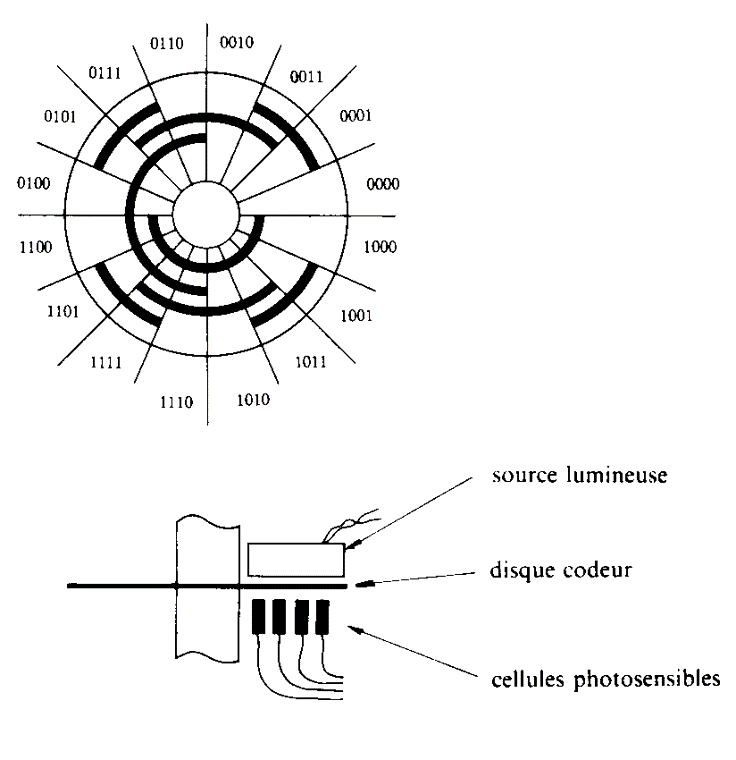
\includegraphics[width=\linewidth]{img/img01}
 \end{center}
\end{minipage}
}}

{\frame{
\frametitle{Définition pour les opérations}
\begin{itemize}
 \item Les \textbf{opérations logiques} sont réalisées en associant des \textbf{tensions} à des variables logiques,
 \item Les \textbf{états et les valeurs logiques} sont représentés par les nombres 0 et 1,
 \item La \textbf{valeur de la variable} est une \textbf{tension électrique} appliquée entre la borne considérée et la masse du montage,
 \item Une \textbf{fonction logique} est représentée par des groupes de variables reliées par des \textbf{opérateurs logiques}, elle ne peut prendre que les valeurs 0 et 1,
 \item La \textbf{table de vérité} est une table qui permet de connaître la valeur de S en fonction des diverses \textbf{combinaisons} possibles des variables d'entrée Ei,
 \item Le \textbf{chronogramme} est le graphe de l'évolution en fonction du temps des variables et des fonctions logiques.
\end{itemize}
}}

\section{Fonctions combinatoires}

{\frame{
\frametitle{Combinatoire ou séquentiel ?}

\begin{minipage}{0.6\linewidth}
\begin{itemize}
 \item Une fonction est dite \textbf{combinatoire} si ses sorties \textbf{ne dépendent que} des combinaisons d'entrée et pas de l'histoire de celles-ci,
 \item A une combinaison de variables d'entrée correspond une seule combinaison des sorties,
 \item Aucune mémoire des états précédents n'est conservée.
\end{itemize}
\end{minipage}\hfill
\begin{minipage}{0.35\linewidth}
\centering 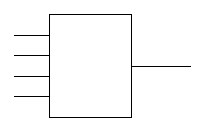
\includegraphics[width=0.7\linewidth]{img/img02}
\end{minipage}

\begin{minipage}{0.6\linewidth}
\begin{itemize}
 \item Une fonction est dite séquentielle si ses sorties \textbf{dépendent} des combinaisons d'entrée et de l'histoire de celles-ci,
 \item A une combinaison de variables d'entrée correspond plusieurs combinaisons des sorties,
 \item Tout ou partie des combinaisons d'entrée et de sortie qui peuvent influencer les sorties de nouvelles combinaisons est conservé.
\end{itemize}
\end{minipage}\hfill
\begin{minipage}{0.35\linewidth}
\centering 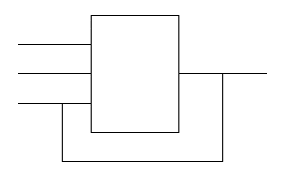
\includegraphics[width=0.7\linewidth]{img/img03}
\end{minipage}
}}


{\frame{
\frametitle{Fonction à une variable logique}

\begin{minipage}{0.6\linewidth}
\begin{itemize}
 \item \textbf{OUI}: $S=E$,
 \item S est \textbf{identique} à E.
\end{itemize}
\end{minipage}\hfill
\begin{minipage}{0.35\linewidth}
\centering 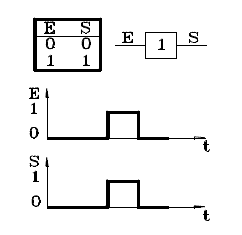
\includegraphics[width=0.7\linewidth]{img/img04}
\end{minipage}

\begin{minipage}{0.6\linewidth}
\begin{itemize}
 \item \textbf{NON}: $S=\overline{E}$,
 \item S est le \textbf{complément} de E.
\end{itemize}
\end{minipage}\hfill
\begin{minipage}{0.35\linewidth}
\centering 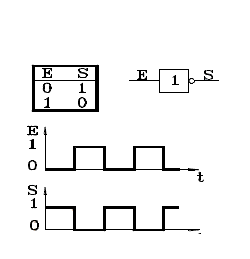
\includegraphics[width=0.7\linewidth]{img/img05}
\end{minipage}
}}

{\frame{
\frametitle{Fonction à deux variables logiques}

\begin{minipage}{0.6\linewidth}
\begin{itemize}
 \item \textbf{OU}: $S=E_1+E_2$,
 \item S est vrai si $E_1$ \textbf{ou} $E_2$ est vrai.
\end{itemize}\vspace{2cm}
\begin{itemize}
 \item \textbf{ET}: $S=E_1.E_2$,
 \item S est vrai si $E_1$ \textbf{et} $E_2$ sont vrai.
\end{itemize}
\end{minipage}\hfill
\begin{minipage}{0.35\linewidth}
\centering 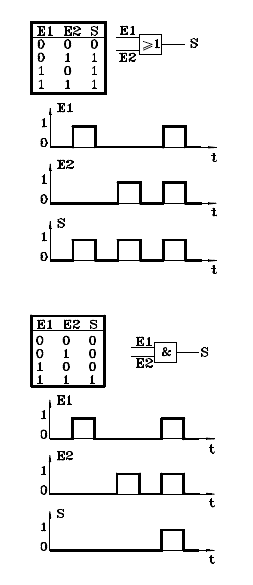
\includegraphics[width=0.7\linewidth]{img/img06}
\end{minipage}
}}

{\frame{
\frametitle{Fonction à deux variables logiques}

\begin{minipage}{0.6\linewidth}
\begin{itemize}
 \item \textbf{NON OU}: $S=\overline{E_1+E_2}$,
 \item S est le \textbf{complément} de $(E_1+E_2)$.
\end{itemize}\vspace{2cm}
\begin{itemize}
 \item \textbf{NON ET}: $S=\overline{E_1.E_2}$,
 \item S est le \textbf{complément} de $(E_1.E_2)$.
\end{itemize}
\end{minipage}\hfill
\begin{minipage}{0.35\linewidth}
\centering 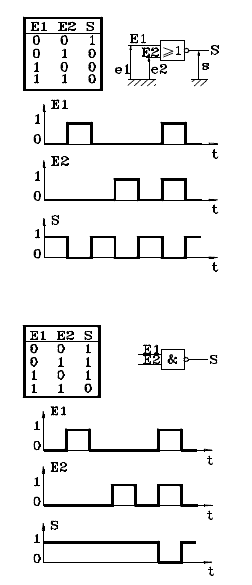
\includegraphics[width=0.7\linewidth]{img/img07}
\end{minipage}
}}

{\frame{
\frametitle{Fonction à deux variables logiques}

\begin{minipage}{0.6\linewidth}
\begin{itemize}
 \item \textbf{OU exclusif}: $S=E_1\oplus E_2$,
 \item $S=E_1.\overline{E_2}+\overline{E_1}.E_2$,
 \item S ne vaut 1 que si les 2 variables d'entrée ont des valeurs différentes: \textbf{anticoïncidence}.
\end{itemize}\vspace{2cm}
\begin{itemize}
 \item \textbf{NON OU exclusif}: $S=\overline{E_1\oplus E_2}$,
 \item $S=\overline{E_1}.\overline{E_2}+E_1.E_2$,
 \item S ne vaut 1 que si les 2 variables d'entrée ont des valeurs identiques: \textbf{coïncidence}.
\end{itemize}
\end{minipage}\hfill
\begin{minipage}{0.35\linewidth}
\centering 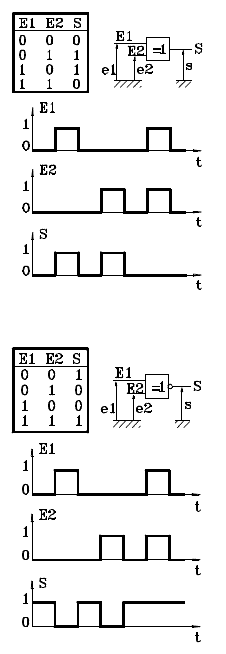
\includegraphics[width=0.6\linewidth]{img/img08}
\end{minipage}
}}

{\frame{
\frametitle{Théorèmes fondamentaux}

\begin{itemize}
 \item identités remarquables: 
  \begin{itemize}
   \item  $1.E=E$, $E+1=1$, $0.E=0$, $E+0=E$,
  \end{itemize}
 \item commutativité:
  \begin{itemize}
   \item  $E_1.E_2=E_2.E_1$, $E_1+E_2=E_2+E_1$,
  \end{itemize}
 \item associativité:
  \begin{itemize}
   \item  $E_1.(E_2.E_3)=(E_1.E_2).E_3$, $E_1+(E_2+E_3)=(E_1+E_2)+E_3$,
  \end{itemize}
 \item distributivité:
  \begin{itemize}
   \item  $E_1.(E_2+E_3)=(E_1.E_2)+(E_1.E_3)$, $E_1+(E_2.E_3)=(E_1+E_2).(E_1+E_3)$,
  \end{itemize}
   \item idempotence:
  \begin{itemize}
   \item  $E+E=E$, $E.E=E$
  \end{itemize}
   \item complémentarité
  \begin{itemize}
   \item  $E+\overline{E}=1$, $E.\overline{E}=0$
  \end{itemize}
   \item absorption
  \begin{itemize}
   \item  $E+E.A=E$.
  \end{itemize}
 \end{itemize}
}}

{\frame{
\frametitle{Théorèmes fondamentaux}

\textbf{Principe de dualité:}

Toute expression logique demeure vraie si l'on remplace '+' par '.' et 0 par 1 et réciproquement (facilement vérifiable pour les expressions précédentes).

\textbf{Théorèmes de De Morgan}
\begin{itemize}
 \item Théorème 1:
 
Le produit logique complémenté de 2 variables booléennes est égal à la somme logique des compléments de ces variables:
\begin{center}
 $\overline{E_1.E_2}=\overline{E_1}+\overline{E_2}$,
\end{center}

 \item Théorème 2:
 
La somme logique complémentée de 2 variables booléennes est égale au produit logique des compléments de ces variables:
\begin{center}
 $\overline{E_1+E_2}=\overline{E_1}.\overline{E_2}$,
\end{center}
 \item Remarque: Ces relations sont généralisables à n variables booléennes.
\end{itemize}
}}

\section{Opérateurs logiques}

{\frame{
\frametitle{Représentation des opérateurs logiques}

\textbf{Emploi d'opérateurs NOR}

\begin{center}
 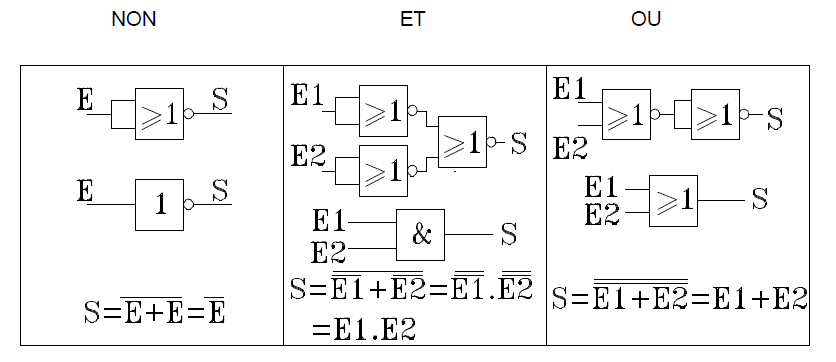
\includegraphics[width=0.9\linewidth]{img/img09}
\end{center}
}}

{\frame{
\frametitle{Représentation des opérateurs logiques}

\textbf{Emploi d'opérateurs NAND}

\begin{center}
 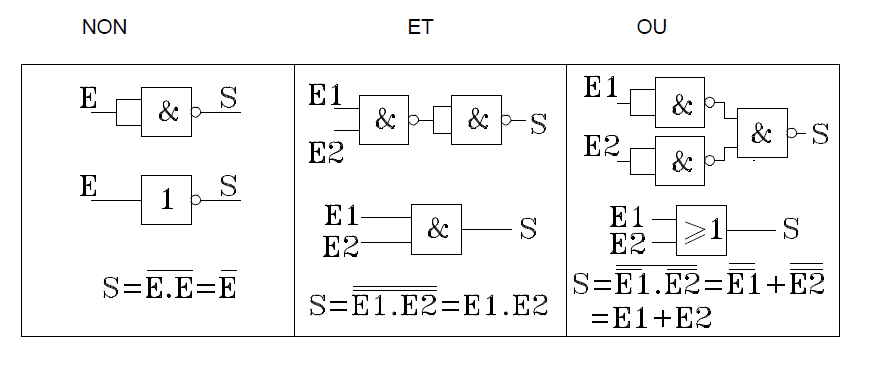
\includegraphics[width=0.9\linewidth]{img/img10}
\end{center}
}}	

{\frame{
\frametitle{Représentation des opérateurs logiques}

\textbf{Exemple}

\begin{itemize}
 \item Soit la forme canonique $S=\overline{E_1}.E_2+E_1.\overline{E_2}$,
\end{itemize}
 \begin{center}
 \begin{tabular}{|c|c|c|}
 \hline
 $E_1$ & $E_2$ & $S$ \\ \hline
 0 & 0 & 0 \\ \hline
 0 & 1 & 1 \\ \hline
 1 & 0 & 1 \\ \hline
 1 & 1 & 0 \\ \hline
 \end{tabular}
 \end{center}
\textbf{Question:} Établir les montages avec des opérateurs NAND et NOR.
}}

{\frame{
\frametitle{Représentation des opérateurs logiques}

\textbf{1\textsuperscript{ère} solution avec opérateurs NAND}

\begin{itemize}
 \item D'après le théorème de De Morgan:
\begin{center}
 $\overline{S}=\overline{E_1.\overline{E_2}+\overline{E_1}.E_2}=\overline{E1.\overline{E2}}.\overline{\overline{E1}.E2}$ \\
 	Donc: $S=\overline{\overline{E1.\overline{E2}}.\overline{\overline{E1}.E2}}$
\end{center}
 \item Ce qui donne la solution suivante avec 5 opérateurs NAND:
\begin{center}
 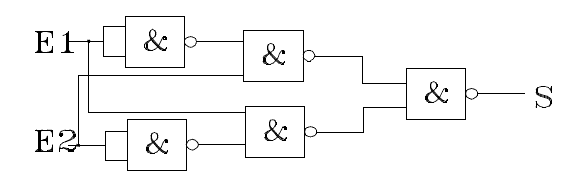
\includegraphics[width=0.9\linewidth]{img/img11}
\end{center}
\end{itemize}
}}

{\frame{
\frametitle{Représentation des opérateurs logiques}

\textbf{2\textsuperscript{ème} solution avec opérateurs NOR}

\begin{itemize}
 \item D'après le théorème de De Morgan:
\begin{center}
$S=E_1.\overline{E_2}+\overline{E_1}.E_2+E_1.\overline{E_1}+E_2.\overline{E_2}=(E_1+E_2).(\overline{E_1}+\overline{E_2})$ \\
D'après le théorème de De Morgan : $\overline{S}=\overline{(E_1+E_2).(\overline{E_1}+\overline{E_2})}=\overline{(E_1+E_2)}+\overline{(\overline{E_1}+\overline{E_2})}$ \\
Donc: $S=\overline{\overline{(E_1+E_2)}+\overline{(\overline{E_1}+\overline{E_2})}}$
\end{center}
 \item Ce qui donne la solution suivante avec 5 opérateurs NOR:
\begin{center}
 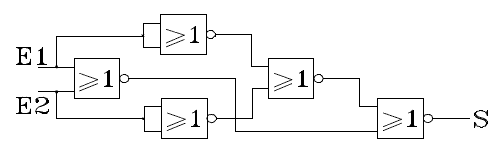
\includegraphics[width=0.9\linewidth]{img/img12}
\end{center}
\end{itemize}
}}

\section{Méthode de Karnaugh}

{\frame{
\frametitle{Méthode de Karnaugh}

\begin{itemize}
 \item La représentation d'une forme canonique sous la forme d'une table de vérité devient \textbf{lourde} dés que le nombre de variables d'entrée est important. Par exemple, 3 variables nécessitent 8 lignes dans la table,
 \item La méthode de \textbf{Karnaugh} permet de simplifier une expression booléenne et de déduire le montage adéquat,
 \item Elle consiste à mettre en évidence le regroupement de termes tel que $A+A.B=A$,
 \item Le codage des états des lignes et des colonnes est binaire réfléchi pour qu'une et une seule variable change d'état d'une case à une case adjacente.
\end{itemize}
}}

{\frame{
\frametitle{Méthode de Karnaugh}

\begin{itemize}
 \item Soit la forme canonique $S=\overline{E_1.E_3+E_2.E_4}$.
 \begin{center}
 $S=\overline{E_1.E_3}.\overline{E_2.E_4}=(\overline{E_1}+\overline{E_3}). (\overline{E_2}+\overline{E_4})=\overline{E_1}.\overline{E_2}+\overline{E_1}.\overline{E_4}+\overline{E_3}.\overline{E_2}+\overline{E_3}.\overline{E_4}$
 \end{center}
 \item D'un point de vue théorique, on a avec 4 variables:\\
	\begin{center}		
	\begin{tabular}{|c|c|c|c|c|}\hline
	\rowcolor{blmr} $E_1.E_2/E_3.E_4$ & 0 0 & 0 1 & 1 1 & 1 0 \\ \hline 
	\rowcolor{bleuc} 0 0 & $\overline{E_1}.\overline{E_2}.\overline{E_3}.\overline{E_4}$ & $\overline{E_1}.\overline{E_2}.\overline{E_3}.E_4$ & $\overline{E_1}.\overline{E_2}.E_3.E_4$  & $\overline{E_1}.\overline{E_2}.E_3.\overline{E_4}$ \\ \hline 
	\rowcolor{blmr} 0 1 & $\overline{E_1}.E_2.\overline{E_3}.\overline{E_4}$ & $\overline{E_1}.E_2.\overline{E_3}.E_4$ & $\overline{E_1}.E_2.E_3.E_4$  & $\overline{E_1}.E_2.E_3.\overline{E_4}$ \\ \hline
	\rowcolor{bleuc} 1 1 & $E_1.E_2.\overline{E_3}.\overline{E_4}$ & $E_1.E_2.\overline{E_3}.E_4$ & $E_1.E_2.E_3.E_4$  & $E_1.E_2.E_3.\overline{E_4}$ \\ \hline
	\rowcolor{blmr} 1 0 & $E_1.\overline{E_2}.\overline{E_3}.\overline{E_4}$ & $E_1.\overline{E_2}.\overline{E_3}.E_4$ & $E_1.\overline{E_2}.E_3.E_4$ & $E_1.\overline{E_2}.E_3.\overline{E_4}$ \\ \hline
	\end{tabular}
	\end{center}
 \item D'un point de vue théorique, on a avec 4 variables:\\
	\begin{center}	
	\begin{tabular}{|c|c|c|c|c|}\hline
	\rowcolor{blmr} $E_1.E_2/E_3.E_4$ & 0 0 & 0 1 & 1 1 & 1 0 \\ \hline 
	\rowcolor{bleuc} 0 0 & 1 & 1 & 1 & 1 \\ \hline 
	\rowcolor{blmr} 0 1 & 1 & 0 & 0 & 1 \\ \hline
	\rowcolor{bleuc} 1 1 & 1 & 0 & 0 & 0 \\ \hline
	\rowcolor{blmr} 1 0 & 1 & 1 & 0 & 0 \\ \hline
	\end{tabular}
	\end{center}
\end{itemize}
}}

{\frame{
\frametitle{Détermination de fonction logique}

\begin{itemize}
 \item La méthode de recherche de l'\textbf{expression minimale} d'une fonction logique $S$ à partir d'un tableau de Karnaugh consiste à rechercher des cases \textbf{adjacentes} comportant des $1$ de sorte qu'un regroupement puisse être opéré dans le but de simplifier $S$,
 \item Les cases extrêmes peuvent être considérées comme adjacentes puisqu'une seule variable change d'état, donc le tableau peut être considéré comme un cylindre vertical ou horizontal,
\begin{center}
 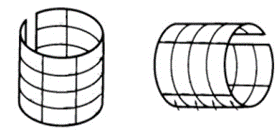
\includegraphics[width=0.3\linewidth]{img/img13}
\end{center}
 \item \textit{Remarque:} Lorsque certains états de la fonction S ne sont \textbf{pas définis}, l'état de la sortie dans le tableau de Karnaugh est symbolisé par une croix (état indifférent). Les croix peuvent être remplacées par des $0$ ou des $1$ pour faciliter au mieux les regroupements.
\end{itemize}
}}

{\frame{
\frametitle{Détermination de fonction logique}

\textbf{Recherche d'octets}

Huit $1$ voisins peuvent être regroupés car 3 variables changent d'état, celles-ci disparaissent dans le terme qui résulte.

\begin{center}
\begin{tabular}{|c|c|c|c|}\hline
 & \cellcolor{blmr} 1 & \cellcolor{blmr} 1 &  \\ \hline 
 & \cellcolor{blmr} 1 & \cellcolor{blmr} 1 &  \\ \hline
 & \cellcolor{blmr} 1 & \cellcolor{blmr} 1 &  \\ \hline
 & \cellcolor{blmr} 1 & \cellcolor{blmr} 1 &  \\ \hline
\end{tabular} \hspace{2cm}
\begin{tabular}{|c|c|c|c|}\hline
\cellcolor{blmr} 1 & & & \cellcolor{blmr} 1  \\ \hline 
\cellcolor{blmr} 1 & & & \cellcolor{blmr} 1  \\ \hline
\cellcolor{blmr} 1 & & & \cellcolor{blmr} 1  \\ \hline
\cellcolor{blmr} 1 & & & \cellcolor{blmr} 1  \\ \hline
\end{tabular}
\end{center}

Exemple: $S=\overline{E_3}$
\begin{center}	
 \begin{tabular}{|c|c|c|c|c|}\hline
  $E_1.E_2/E_3.E_4$ & 0 0 & 0 1 & 1 1 & 1 0 \\ \hline 
  0 0 & 1 & 1 & 0 & 0 \\ \hline 
  0 1 & 1 & 1 & 0 & 0 \\ \hline
  1 1 & 1 & 1 & 0 & 0 \\ \hline
  1 0 & 1 & 1 & 0 & 0 \\ \hline
 \end{tabular}
\end{center}
}}

{\frame{
\frametitle{Détermination de fonction logique}

\textbf{Recherche de quartets}

Quatre $1$ voisins peuvent être regroupés car deux variables changent d'état, celles-ci disparaissent dans le terme qui résulte.


\begin{center}
\begin{tabular}{|c|c|c|c|}\hline
 & & \cellcolor{blmr} 1 &  \\ \hline 
 & & \cellcolor{blmr} 1 &  \\ \hline
 & & \cellcolor{blmr} 1 &  \\ \hline
 & & \cellcolor{blmr} 1 &  \\ \hline
\end{tabular}
\begin{tabular}{|c|c|c|c|}\hline
 &  &  &  \\ \hline 
 &  & \cellcolor{blmr} 1 & \cellcolor{blmr} 1  \\ \hline
 &  & \cellcolor{blmr} 1 & \cellcolor{blmr} 1  \\ \hline
 &  &  &  \\ \hline
\end{tabular}
\begin{tabular}{|c|c|c|c|}\hline
\cellcolor{blmr} 1 & & & \cellcolor{blmr} 1  \\ \hline 
					& & &   				   \\ \hline
				    & & &   			  	   \\ \hline
\cellcolor{blmr} 1 & & & \cellcolor{blmr} 1  \\ \hline
\end{tabular}
\begin{tabular}{|c|c|c|c|}\hline
 					 &  &  &  \\ \hline 
 \cellcolor{blmr} 1 &  &  &  \cellcolor{blmr} 1  \\ \hline
 \cellcolor{blmr} 1 &  &  &  \cellcolor{blmr} 1  \\ \hline
 					 &  &  &  \\ \hline
\end{tabular}
\end{center}

Exemple: $S=E_1.E_2+\overline{E_2}.\overline{E_4}$
\begin{center}	
 \begin{tabular}{|c|c|c|c|c|}\hline
  $E_1.E_2/E_3.E_4$ & 0 0 & 0 1 & 1 1 & 1 0 \\ \hline 
  0 0 & 1 & 0 & 0 & 1 \\ \hline 
  0 1 & 0 & 0 & 0 & 0 \\ \hline
  1 1 & 1 & 1 & 1 & 1 \\ \hline
  1 0 & 1 & 0 & 0 & 1 \\ \hline
 \end{tabular}
\end{center}
}}
{\frame{
\frametitle{Détermination de fonction logique}

\textbf{Recherche de doublets}

Deux $1$ voisins peuvent être regroupés car une seule
variable change d'état, celle-ci disparaît dans le terme
qui résulte.


\begin{center}
\begin{tabular}{|c|c|c|c|}\hline
 &  & 					  &  \\ \hline 
 &  & \cellcolor{blmr} 1 &  \\ \hline
 &  & \cellcolor{blmr} 1 &  \\ \hline
 &  & 					  &  \\ \hline
\end{tabular} \hspace{2cm}
\begin{tabular}{|c|c|c|c|}\hline
\cellcolor{blmr} 1 & & & \cellcolor{blmr} 1  \\ \hline 
					& & & 					   \\ \hline
					& & & 					   \\ \hline
					& & & 					   \\ \hline
\end{tabular}
\end{center}

Exemple: $S=\overline{E_1}.\overline{E_2}.\overline{E_3}+\overline{E_2}\overline{E_3}.E_4+E_2.E_3.E_4+E_1.E_3.\overline{E_4}$
\begin{center}	
 \begin{tabular}{|c|c|c|c|c|}\hline
  $E_1.E_2/E_3.E_4$ & 0 0 & 0 1 & 1 1 & 1 0 \\ \hline 
  0 0 & 1 & 1 & 0 & 0 \\ \hline 
  0 1 & 0 & 0 & 1 & 0 \\ \hline
  1 1 & 0 & 0 & 1 & 1 \\ \hline
  1 0 & 0 & 1 & 0 & 1 \\ \hline
 \end{tabular}
\end{center}
}}

{\frame{
\frametitle{Conclusion}

\begin{savoir}
Vous devez être capables :
\begin{itemize}
 \item de manipuler des équations logiques,
 \item de manipuler des fonctions combinatoires,
 \item de concevoir un câblage de portes logiques.
\end{itemize}
\end{savoir}

\begin{prob}
Il est nécessaire d'utiliser d'autres formes de représentation d'un mécanisme.
\begin{itemize}
 \item \textit{Problème: Comment concevoir une commande séquentielle}
 \item \textbf{Perspectives}: Réaliser des algorithmes séquentiels capables de piloter le comportement d'un système.
\end{itemize}
\end{prob}
}}


\end{document}